\documentclass[12pt]{article}

\usepackage{fullpage}
\usepackage{multicol,multirow}
\usepackage{tabularx}
\usepackage{listings}
\usepackage{pgfplots}
\usepackage[utf8]{inputenc}
\usepackage[russian]{babel}
\usepackage{pgfplots}
\usepackage{tikz}
\usepackage{graphicx}


\begin{document}

% \newpage
% \begin{center}
% {\bfseries ФЕДЕРАЛЬНОЕ ГОСУДАРСТВЕННОЕ БЮДЖЕТНОЕ ОБРАЗОВАТЕЛЬНОЕ\\
% УЧРЕЖДЕНИЕ ВЫСШЕГО ОБРАЗОВАНИЯ\\
% «МОСКОВСКИЙ АВИАЦИОННЫЙ ИНСТИТУТ\\
% (НАЦИОНАЛЬНЫЙ ИССЛЕДОВАТЕЛЬСКИЙ УНИВЕРСИТЕТ)»}
% \vspace{1cm}

% Журнал лабораторных работ
% \vspace{6em}

% \vspace{\fill}

% \begin{center}
% Москва 2024
% \newpage
% \end{center}

\section*{Лабораторная работа №1\, по курсу компьютерной графики}

\textbf{Тема:} Основы 2D-графики и трансформаций\\
\\
\textbf{Задача:} Научиться работать с графическим API для отрисовки 2D-примитивов, освоить основные 2D-трансформации (перемещение, масштабирование, поворот) и изучить алгоритмы построения 2D-кривых. \\
\\
\textbf{Вариант:} 2. Отрисовка прямоугольника с трансформациями\\
Создайте программу, которая отрисовывает прямоугольник.\\
Реализуйте возможность изменения положения, угла поворота и масштабирования
прямоугольника.\\
Управляйте трансформациями с помощью клавиатуры.\\
Дополнительно: Добавьте возможность изменять цвет прямоугольника в зависимости от
направления трансформации

\subsection*{1 Решение}

Для выполнения этой лабораторной работы я использовал библиотеку SFML и пользовался ее возможностями рисовать фигуру и всячески ее трансформировать.
Я смог реализовать перемещение на стрелочках, масштабирование на клавишах W и S, и изменение угла на клавишах A и D.
В процессе решения задачи я решил ограничить движение фигуры внутри пространства окна, чтобы она не заходила за гарницу.
Для этого мне пришлось использовать простые математические формулы, однако для корректной работы понадобилось задебажить программу.
Поэтому я решил написать часть кода, которая будет выводить Debug меню с информацией о фигуре по нажатии кнопки U.
Для этого воспользовался библиотекой filesystem для получения информации о папке, в которой исполняется программа, дабы подгрузить шрифты.
Потом я сделал дополнительное задание с изменением цвета при трансформации. Для этого сделал зависимость Red и Blue в цветовом пространстве от размера и угла поворота соответственно. 


\begin{figure}[h]

\centering

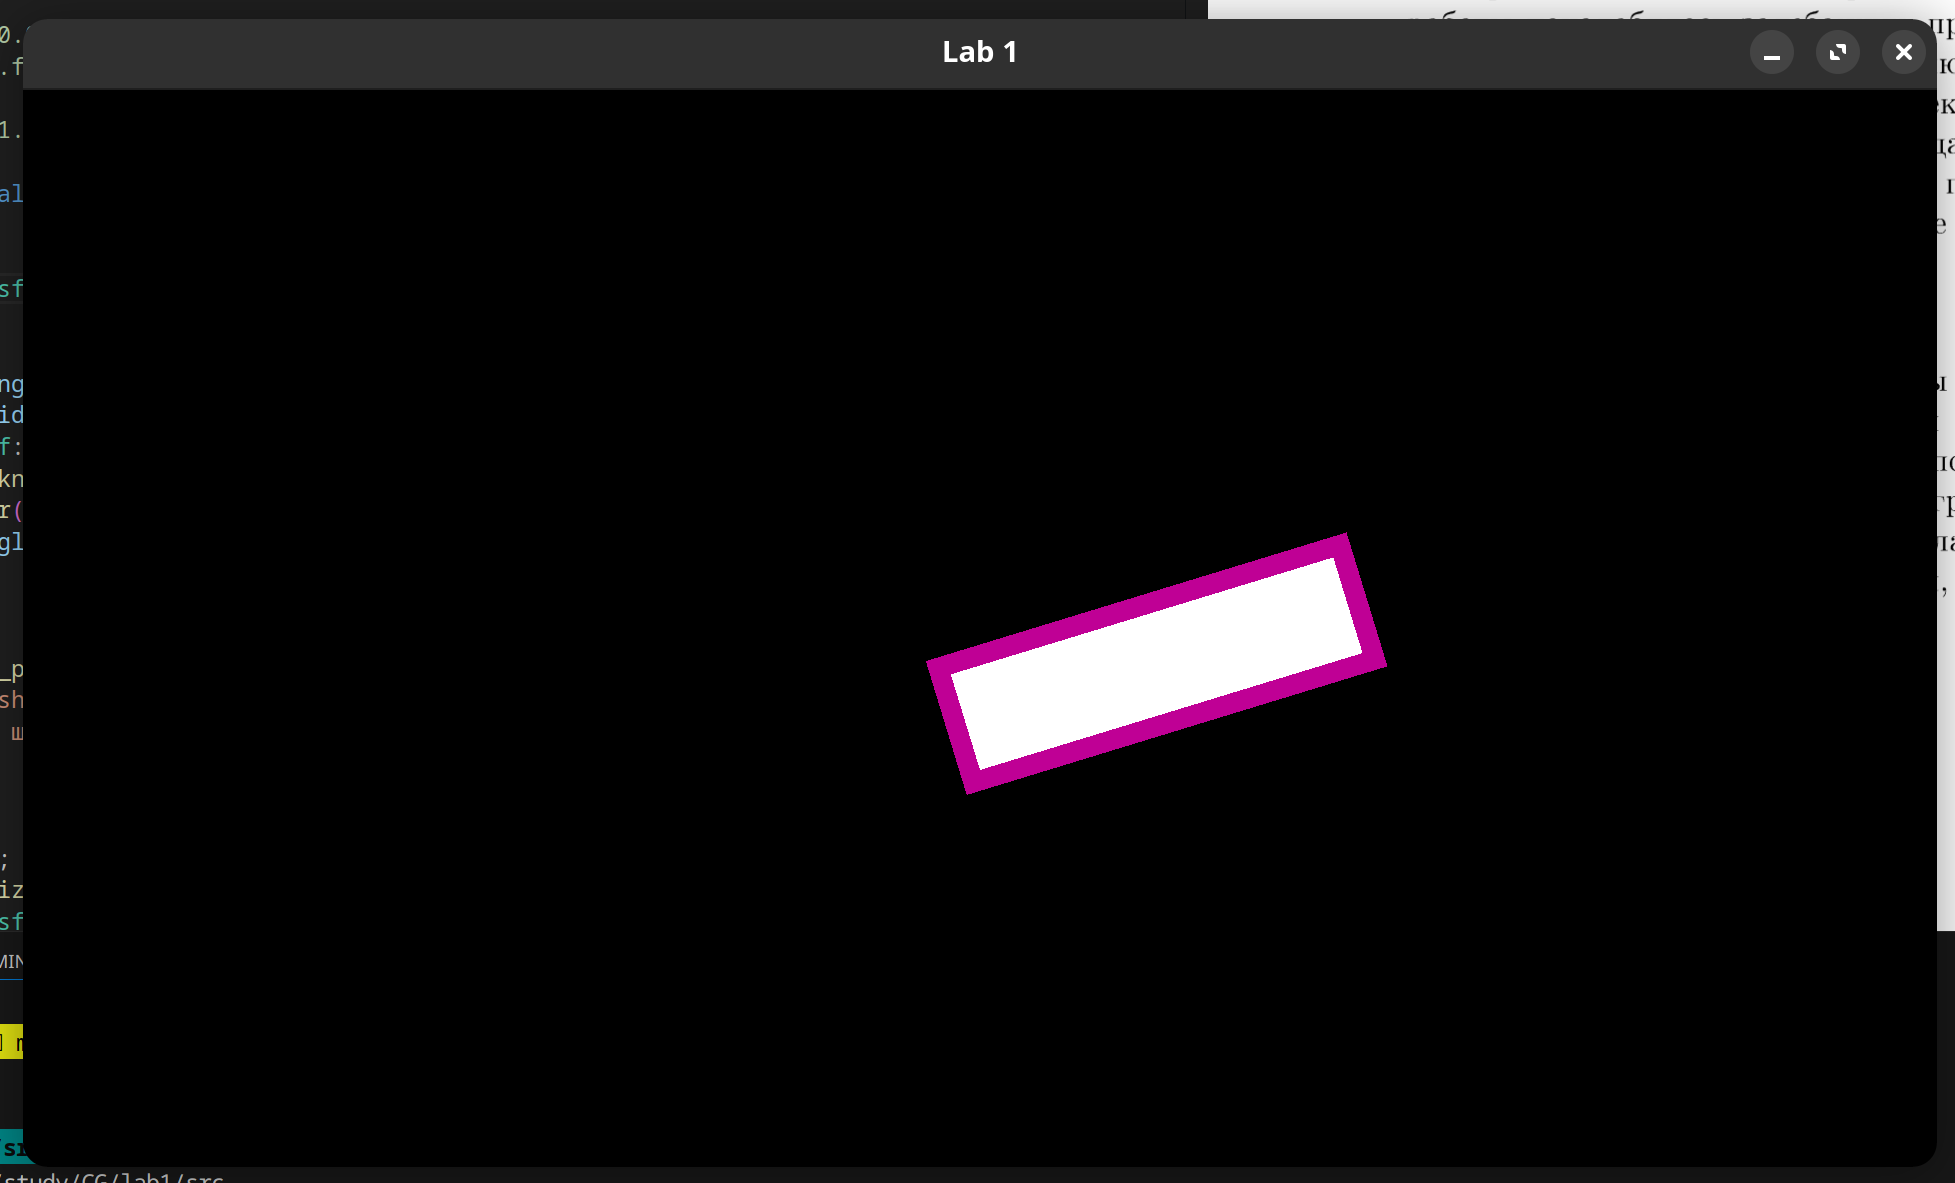
\includegraphics[width=0.8\linewidth]{image.png}

\caption{Пример работы программы}

\label{fig:mpr}

\end{figure}


\subsection*{2 Вывод}

Целью работы было освоение работы с графическим API для отрисовки 2D-примитивов, изучение основных трансформаций (перемещение, масштабирование, поворот) и применение их на практике.
В ходе выполнения лабораторной работы была изучена часть библиотеки SFML для реализации графического интерфейса и работы с графикой. 
По итогу, выполненная работа позволила не только овладеть основными аспектами работы с 2D-графикой и трансформациями, но и применить полученные знания на практике.
\end{document}
